\subsection{State}

Lo \textbf{state diagram} descrive entità/oggetti il cui comportamento può cambiare dinamicamente nel tempo in relazione a determinati eventi o messaggi ricevuti.

Se la risposta dell'oggetto a uno stimolo esterno non dipende unicamente dal suo stato corrente (valore dei campi), ma anche dalla sua storia (azioni passate eseguite in risposta a messaggi precedenti), si dice che l'oggetto possiede degli \textbf{stati di controllo}.

\paragraph{Automa a stati finiti} Se il numero di possibili risposte alle sollecitazioni è finito, l'oggetto possiede un \textbf{automa a stati finiti} (es. iterator), ovvero un grafo orientato i cui nodi sono stati di controllo e i cui archi rappresentano le \textbf{transizioni di stato}.
Nell'approccio object-oriented un automa a stati finiti è associato a una classe e modella in maniera formale il comportamento delle sue istanze partendo da una specifica informale.

\paragraph{Stato iniziale} Lo stato di controllo in cui l'oggetto viene a trovarsi subito dopo la creazione: viene specificato tramite una \textbf{pseudo-transizione} che emana da un cerchietto nero (\textit{pseudo-stato}).

\paragraph{Stati finali} Nodi dai quali non si hanno transizioni. Una transizione di stato è causata da un evento (\textit{trigger}). Si possono specificare delle \textbf{azioni} (operazioni atomiche non interrompibili). A seconda del modo distinguiamo fra:
\begin{itemize}
    \item \textbf{1. Automi di Mealy}: le azioni sono associate alle transizioni. Un'azione viene eseguita SEMPRE E SOLO in risposta al trigger della transizione a cui è associata;
    \item \textbf{2. Automi di Moore}: le azioni sono associate agli stati. Un'azione viene eseguita quando l'automa si trova nello stato di controllo a cui è associata, a prescindere dalla transizione che ha portato in quello stato.
\end{itemize}

\begin{figure}[H]
    \centering
    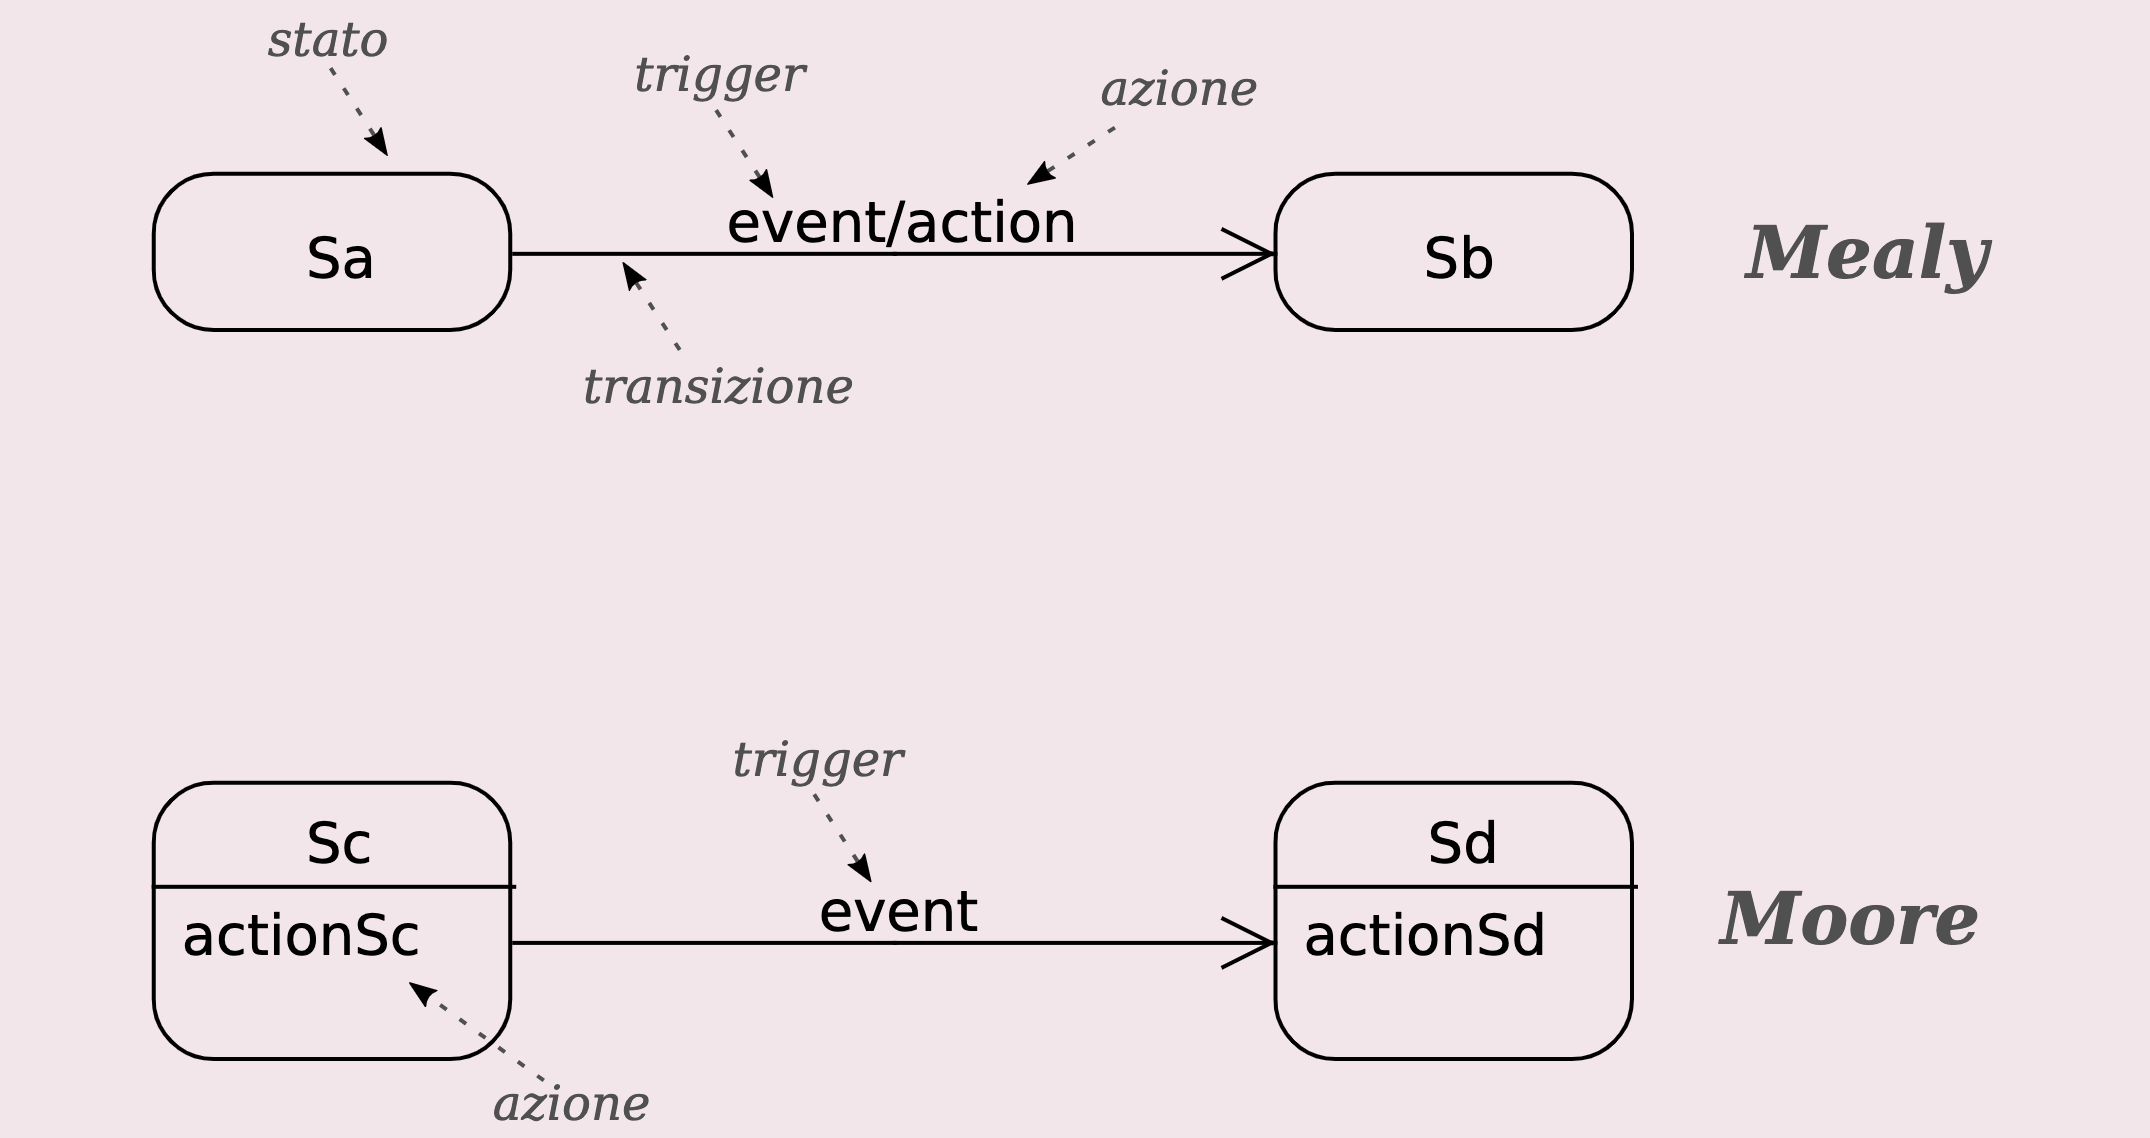
\includegraphics[width=0.8\linewidth]{assets/UML/state/state1.png}
    \caption{I due formalismi sono equivalenti: è sempre possibile trasformare un automa di Mealy in un automa di Moore e viceversa (il numero di stati potrebbe essere diverso)}
\end{figure}

\begin{figure}[H]
    \centering
    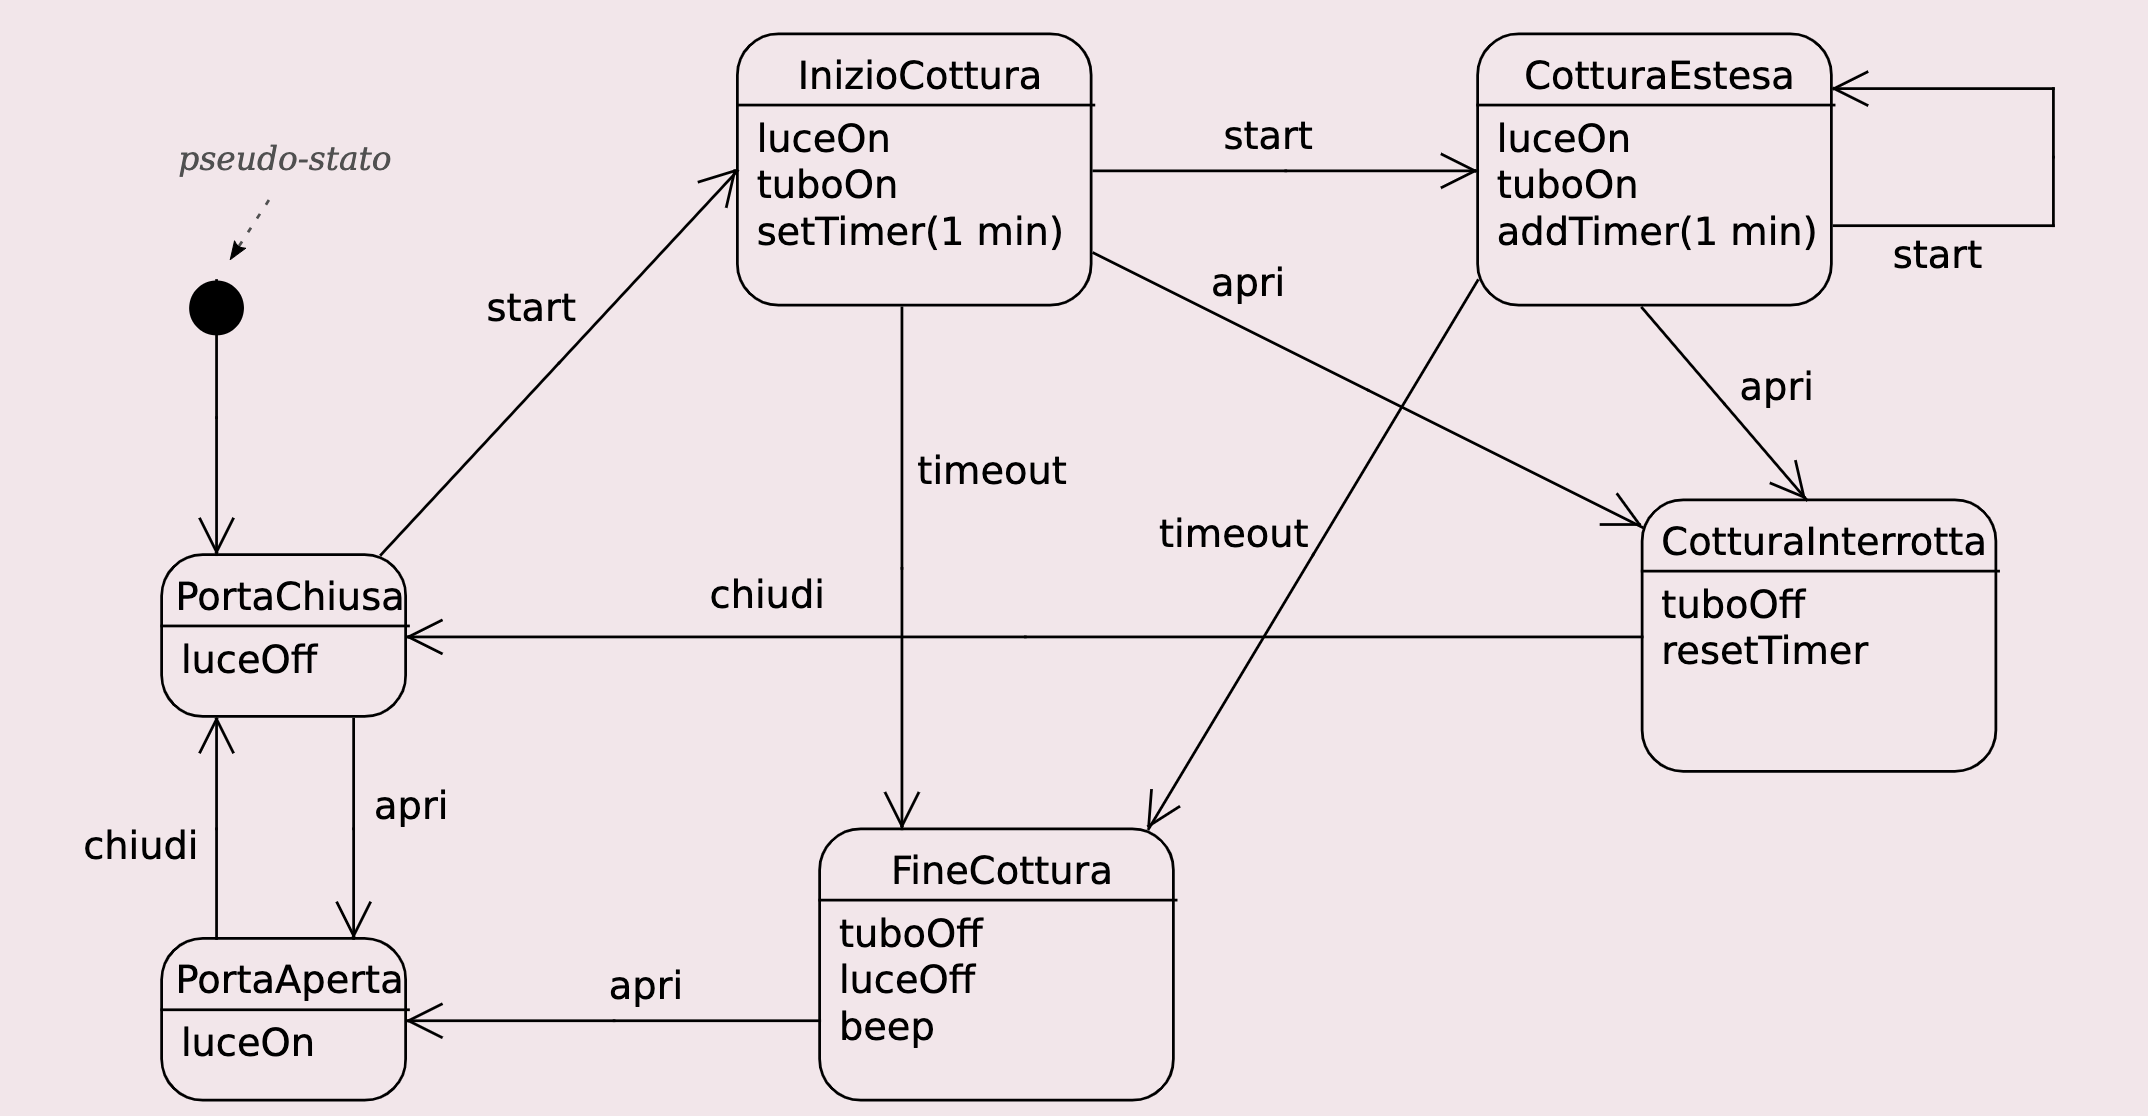
\includegraphics[width=1\linewidth]{assets/UML/state/state2.png}
    \caption{Esempio di automa: forno}
\end{figure}

\paragraph{State Chart} Sono una generalizzazione degli automi a stati finiti; rispetto ad essi consentono di modellare situazioni più complesse.

\begin{figure}[H]
    \centering
    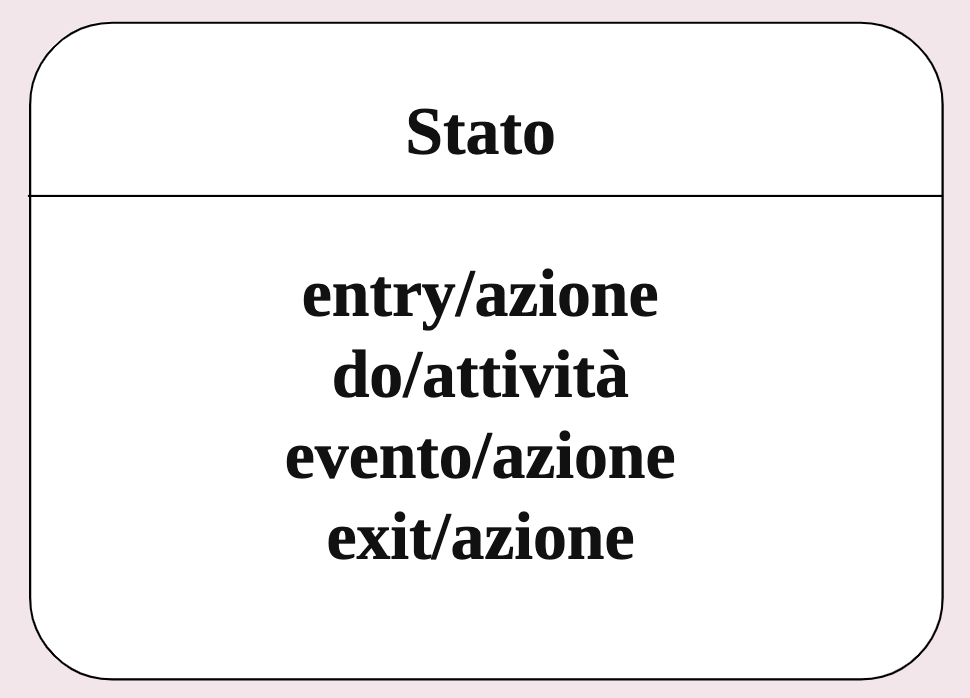
\includegraphics[width=0.25\linewidth]{assets/UML/state/state3.png}
    \caption{Rappresentazione di uno stato di controllo in uno state chart}
\end{figure}

\paragraph{Entry action} Azione triggerata entrando nello stato. Non va confusa con le \textit{attività interne} (non atomiche, interrotte all'uscita dallo stato).

\paragraph{Exit action} Azione triggerata uscendo dallo stato. Si parla di \textit{transizione interna} quando l'oggetto esegue un'operazione rispetto a un evento, ma senza uscire dallo stato. Si parla di \textit{transizione riflessiva} quando l'azione comporta il trigger di entrambe una entry action ed una exit action che riportano lo stato come era inizialmente (AUTOANELLO).

Gli state chart consentono di corredare i trigger con parametri e guardie (condizioni booleane in funzione dello stato corrente dell'oggetto e/o dei parametri ricevuti):

$$evento(parametro)\ [guardia]/azione$$

L'azione verrà eseguita se si verifica il trigger e se allo stesso tempo è vera la guardia. Fra le possibili azioni l'oggetto ha la facoltà di triggerare un altro oggetto (target).

$$send\ target.evento(parametri)$$

Scrivere dentro uno stato "evento/skip" specifica all'automa di ignorare il trigger quando si trova in quello stato.

Gli state chart consentono di modellare delle gerarchie annidando gli stati di controllo: ogni stato è contenuto in uno stato di livello gerarchico superiore (\textbf{\textit{superstato}}) che può a sua volta contenere più stati di livello gerarchico inferiore (\textbf{\textit{sottostati}}). Si dice \textbf{\textit{foglia}} uno stato privo di sottostati. Uno state chart in cui tutti gli stati sono sullo stesso piano gerarchico viene detto \textbf{\textit{piatto}}.

\begin{figure}[H]
    \centering
    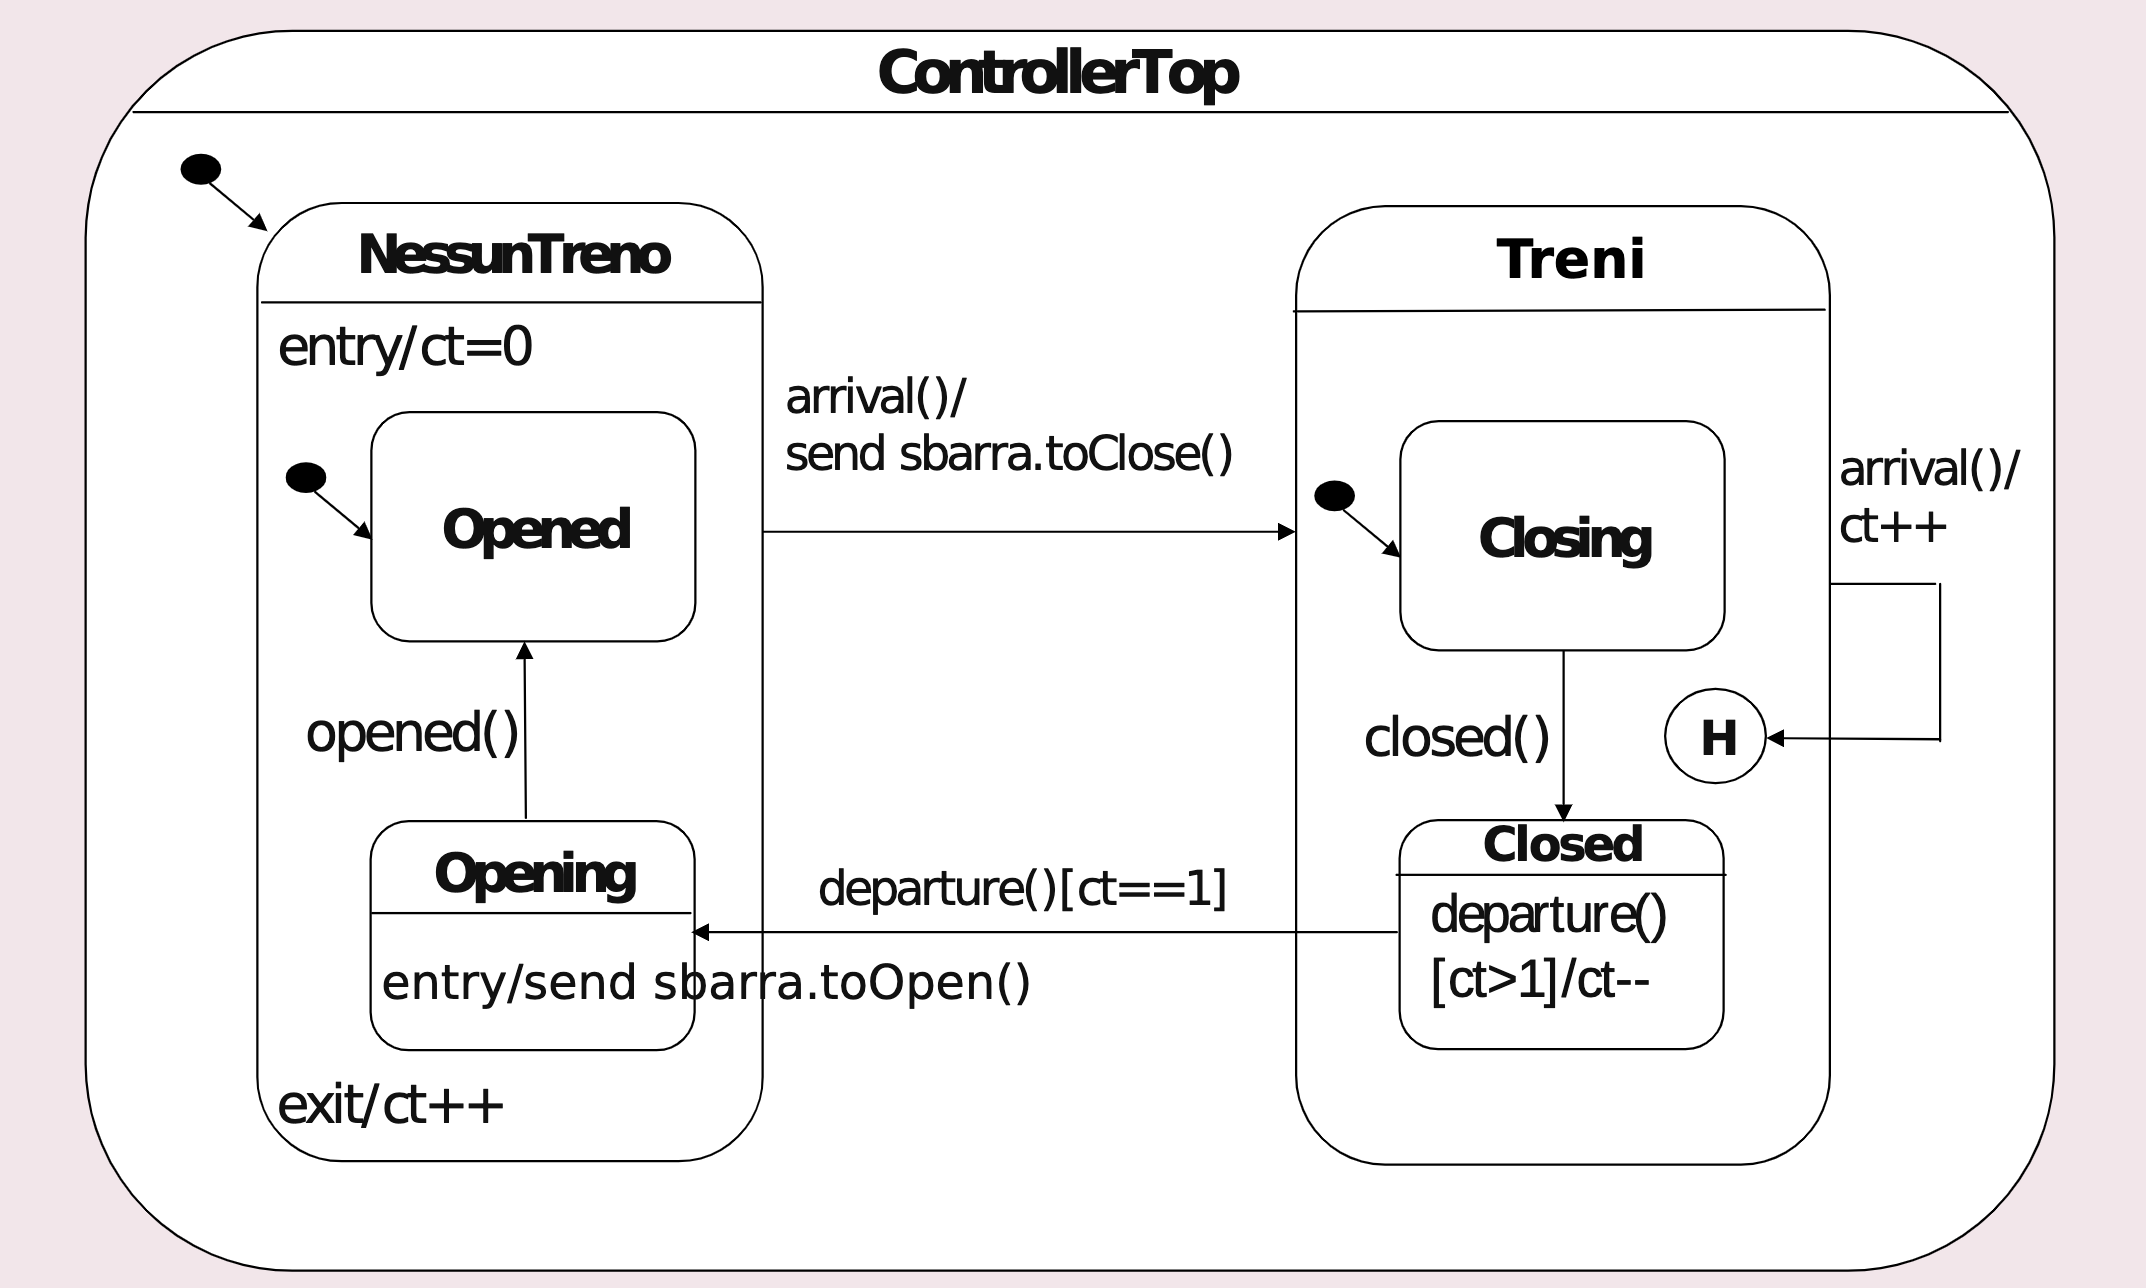
\includegraphics[width=1\linewidth]{assets/UML/state/state4.png}
    \caption{Esempio di state chart: controller di un treno}
\end{figure}

Per ogni stato non foglia una pseudo-transizione indica qual è il sottostato iniziale. Si definisce "configurazione" dell'automa il percorso che va dallo stato di più alto livello gerarchico fino allo stato foglia attuale. Nell'esempio, la configurazione iniziale dell'automa è la seguente:

$$ControllerTop.NessunTreno.Opened$$

\newpage

\paragraph{OR-decomposition} Lo stato foglia attuale è sufficiente a definire univocamente la configurazione corrente dell'automa. Questo perché si applica il \textbf{principio dell'OR esclusivo} (XOR): in ogni stato NON foglia, l'automa deve trovarsi in uno e uno solo dei possibili sottostati.

Si definisce \textbf{transizione di gruppo} quella che parte da uno stato non foglia: può essere triggerata a prescindere dal sottostato specifico in cui si trova l'automa. 

Un \textbf{connettore di storia} è un elemento posto all'interno di uno stato di controllo per consentire all'automa di memorizzare, quando si trova in quello stato, la configurazione corrente. Tornando nello stato, l'automa non assumerà la configurazione di default, bensì quella memorizzata nel connettore. Esistono due tipi di connettori di storia:
\begin{itemize}
    \item \textbf{Storia superficiale (H)}: memorizza la configurazione dallo stato di livello gerarchico più alto fino al livello dei sottostati dello stato con il connettore;
    \item \textbf{Storia profonda (H*)}: memorizza la configurazione dallo stato di livello gerarchico più alto fino allo stato foglia corrente, dunque scendendo in profondità oltre i sottostati dello stato contenente il connettore.
\end{itemize}

In generale, i connettori di storia dovrebbero avere anche una transizione uscente verso un sottostato del macrostato in cui sono contenuti, in modo da poter essere attivati quando l'automa si trova in quello stato. In sua assenza e in assenza di memoria si raggiunge lo stato di default.

Sfruttando il principio di modularità, è possibile definire la gerarchia di uno solo dei possibili stati di controllo, astraendo dai dettagli interni degli altri stati. La presenza di stati non ancora definiti che sono punto di partenza/arrivo di transizioni è segnalata con un cosiddetto \textbf{state stub}.

\newpage

\begin{figure}[H]
    \centering
    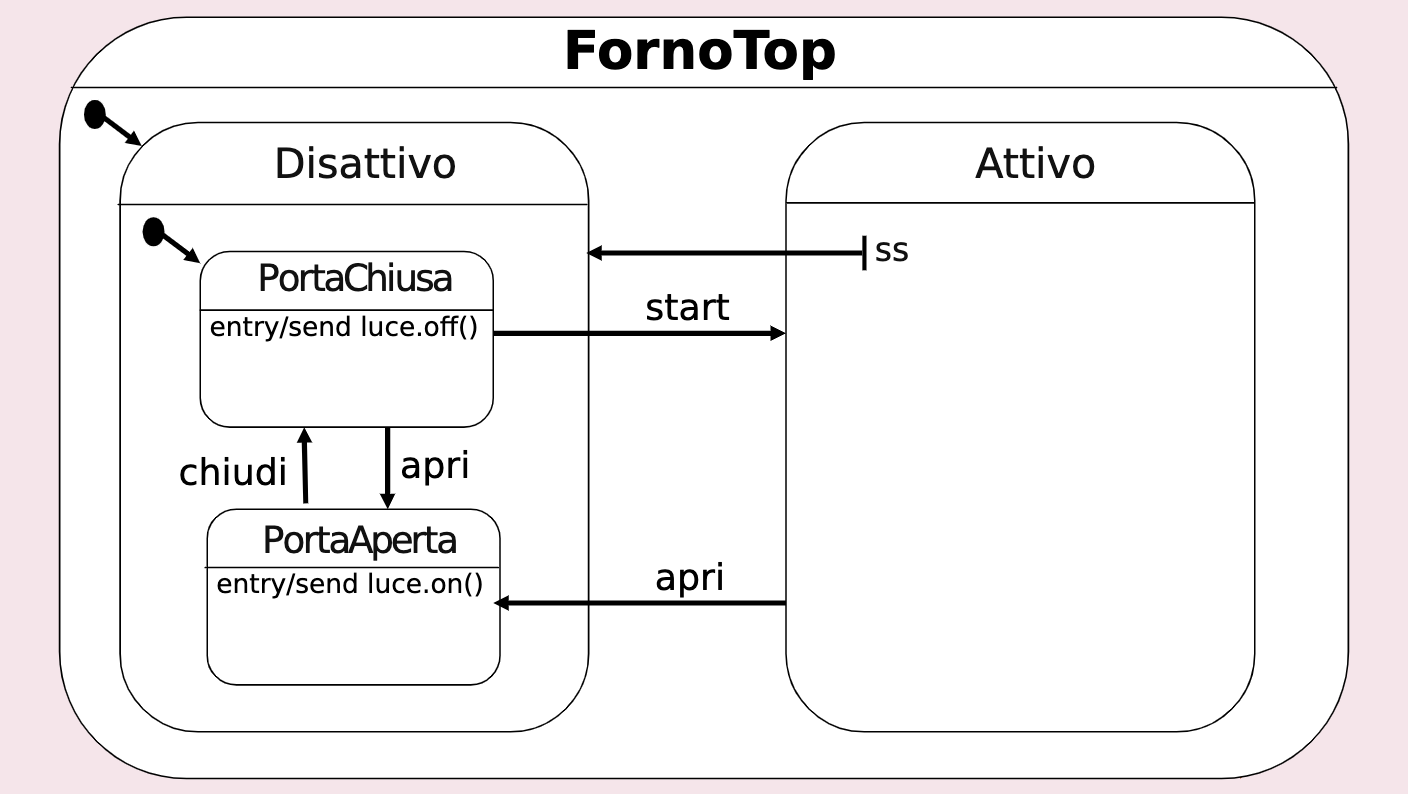
\includegraphics[width=0.75\linewidth]{assets/UML/state/state5.png}
    \caption{Esempio di statechart per il Forno}
\end{figure}

\begin{figure}[H]
    \centering
    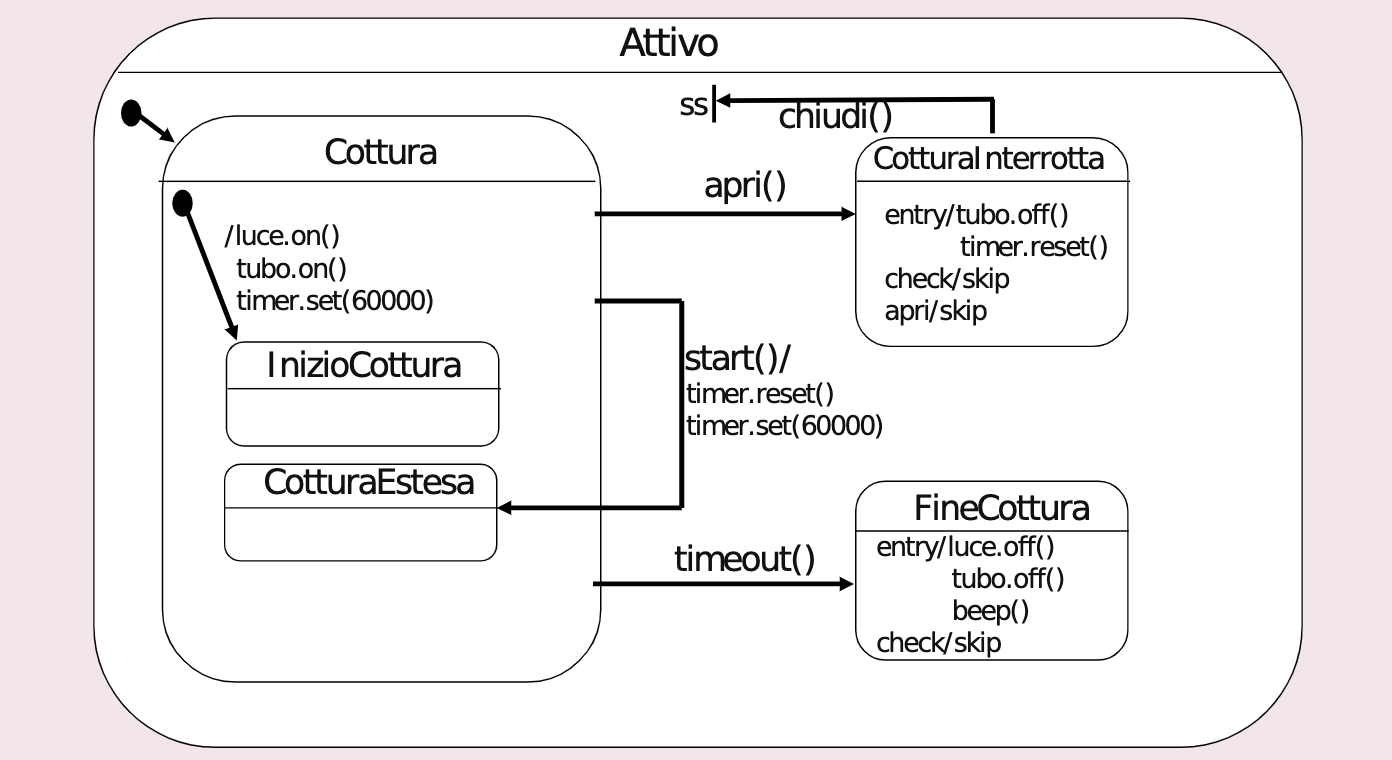
\includegraphics[width=0.75\linewidth]{assets/UML/state/state6.png}
    \caption{Definizione del macrostato "Attivo"}
\end{figure}

\begin{figure}[H]
    \centering
    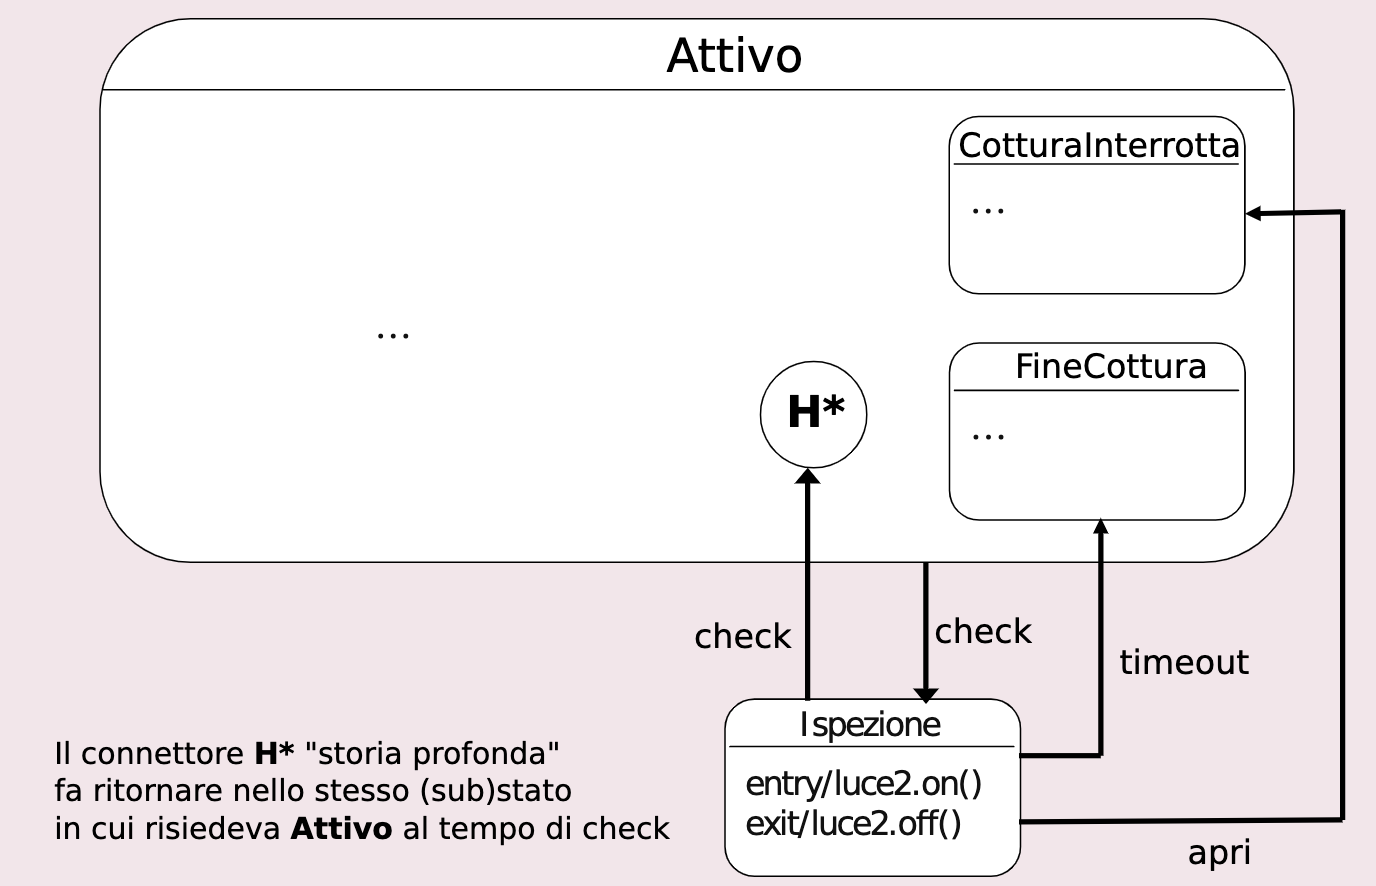
\includegraphics[width=0.75\linewidth]{assets/UML/state/state7.png}
    \caption{Esempio di stato ispezione}
\end{figure}

\newpage

\paragraph{Nota} Per via del concetto di configurazione, in una transizione di stato è necessario individuare:

\begin{itemize}
    \item \textbf{Exit path}: elenco degli stati di controllo da cui si esce, partendo dallo stato sorgente della transizione e risalendo fino al \textbf{Minimum Common Ancestor} (MCA) con lo stato di destinazione (MCA escluso). Si devono eseguire le exit action di tutti gli stati attraversati.
    \item \textbf{Entry path}: elenco degli stati di controllo in cui si entra, partendo dall'MCA (escluso) e scendendo fino allo stato destinazione della transizione. Si devono eseguire tutte le entry action degli stati attraversati.
\end{itemize}

L'MCA è il superstato di livello gerarchico più piccolo che contenga sia la destinazione che la sorgente della transizione.

\subsubsection{Estendere lo state diagram}

Si possono includere negli state chart elementi tipici di un activity diagram: es. punti decisionali (rombi) che pongono due o più transizioni in alternativa. Si può introdurre un'attività (non atomica, interrompibile) in uno stato con la sintassi:

$$do:activity\_name$$

Uno stato con un'attività interna o con eventi processati localmente allo stato può essere scomposto in più sottostati. È possibile triggerare una transizione non con un evento esterno, bensì tramite la maturazione di una condizione internamente all'oggetto:

$$when\ condition$$

Ancora, il trigger della transizione potrebbe essere un \textit{evento di tempo}:

$$after\ time\_expression$$

\newpage

\paragraph{AND-decomposition} Lo stato foglia attuale NON è sufficiente a definire univocamente la condizione corrente dell'automa. In ogni stato NON foglia, l'automa può trovarsi contemporaneamente in due o più possibili sottostati. Lo stato viene diviso in \textit{regioni} parallele e concorrenti.

\begin{figure}[H]
    \centering
    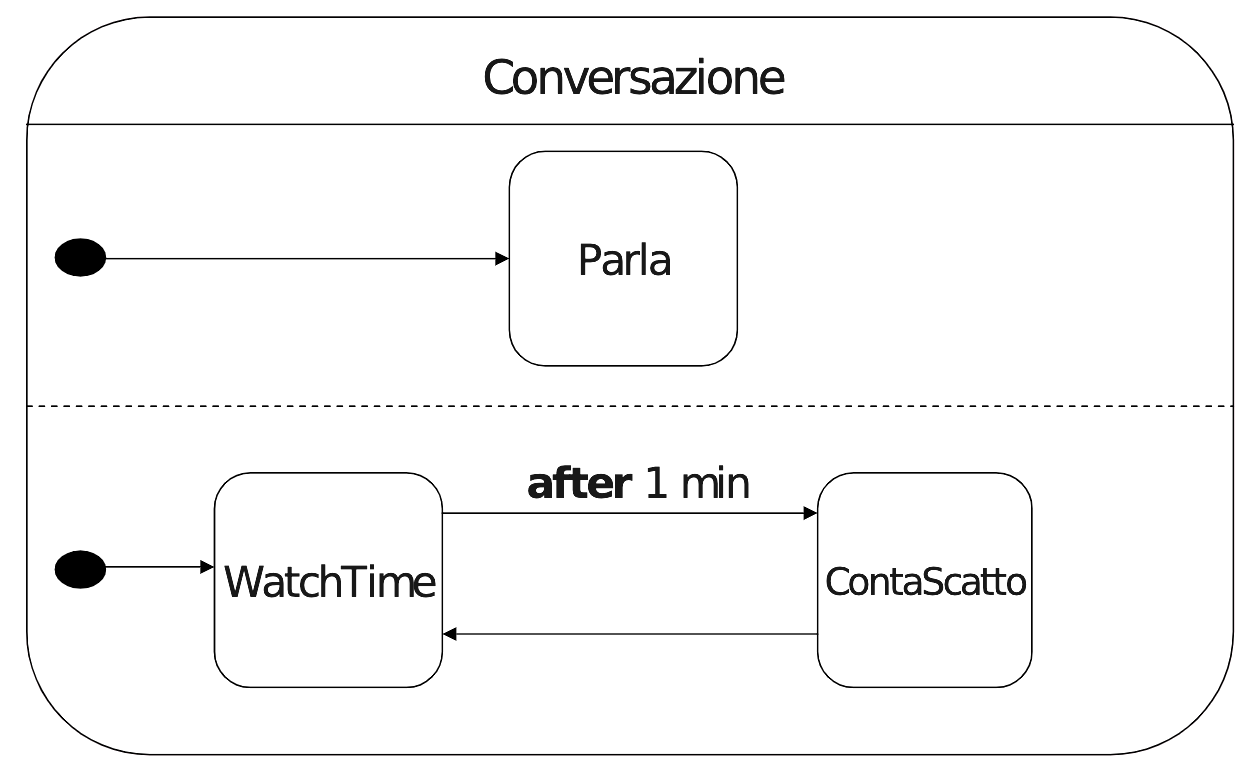
\includegraphics[width=0.7\linewidth]{assets/UML/state/state8.png}
\end{figure}

Nell'esempio, la configurazione iniziale è:

$$Conversazione.Parla|WatchTime$$ 

Sottostati paralleli implicano l'esistenza di thread multipli in uno stesso oggetto (occorre adottare meccanismi di mutua esclusione per proteggere i dati condivisi).

Le transizioni nei due stati paralleli possono essere sincronizzate introducendo delle \textbf{barre di sincronizzazione} e degli \textbf{pseudo-stati di sincronismo} (synch state): l'avanzamento in un sottostato può avvenire solo se nello stato parallelo si è raggiunto un certo punto.

\begin{figure}[H]
    \centering
    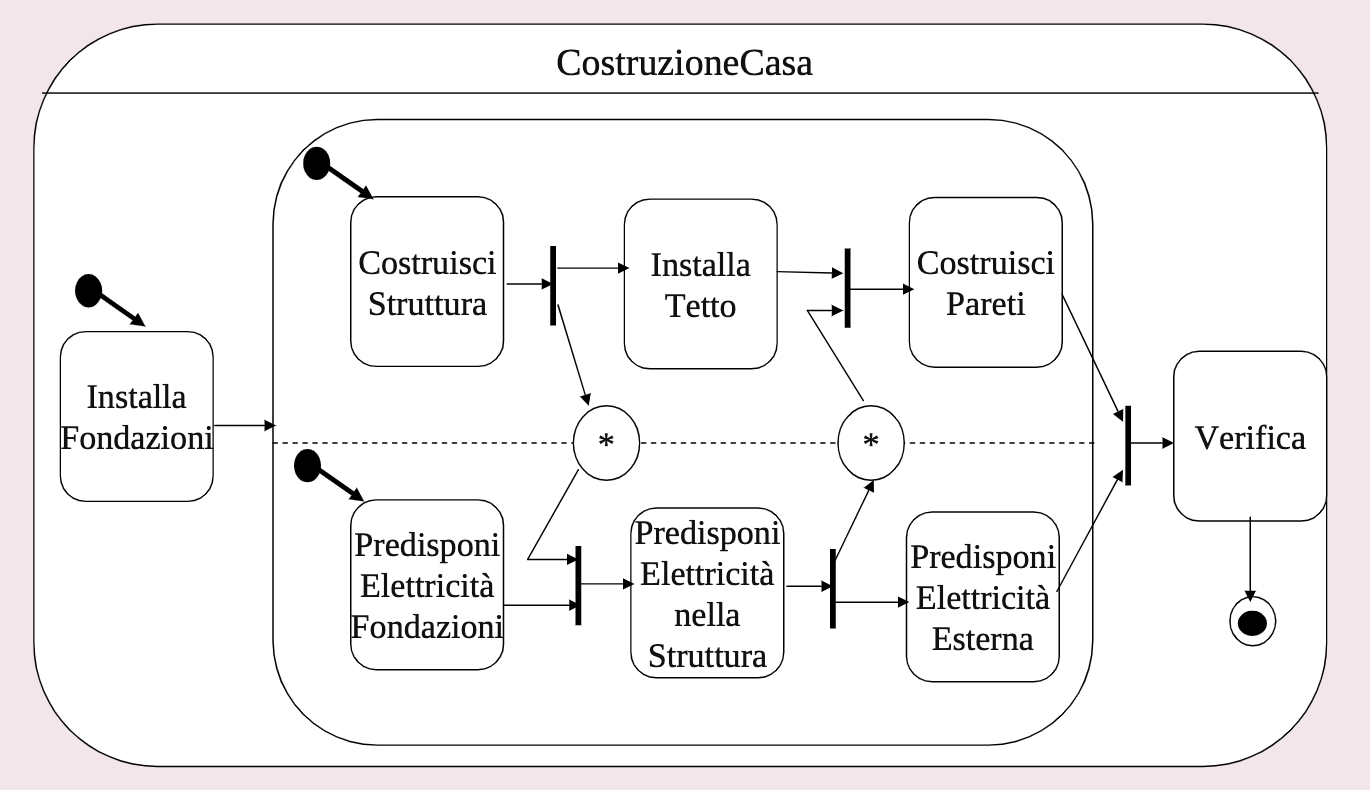
\includegraphics[width=0.7\linewidth]{assets/UML/state/state9.png}
\end{figure}

\newpage
